\section{Parameter-Update Sparsity and Teacher Alignment}
\label{sec:subnetworks}

We examine numerical precision and shared optimizer state when interpreting concentrated checkpoint changes \citep{yu2026denseupdates} and teacher-update alignment.

\subsection{BF16 rounding hides widespread FP32 changes}

Joint training changes about 97\% of FP32 master weights. After BF16 rounding, only 7--9\% of weights differ visibly from initialization under sampled-token or top-64 supervision with equal response weighting (Figure~\ref{fig:subnetwork_overview}a). Small updates are widespread in FP32 and disappear when the weights are stored in BF16.

The precision effect also extends to the concentration of update magnitude. About one third of FP32 coordinates carry 90\% of squared cumulative change, compared with about 4\% of BF16 coordinates. We count unique model coordinates whose displacement from initialization is nonzero, and rank squared displacements to find the smallest coordinate fraction carrying 90\% of the total. Both statistics use the update-500 FP32 master weights and their BF16 stored counterparts.

Loss averaging provides a further comparison between parameter changes and performance. Under top-64 supervision, the averaging rules produce different fractions of changed BF16 weights while reaching similar final mean scores.

\begin{figure}[t]
\centering
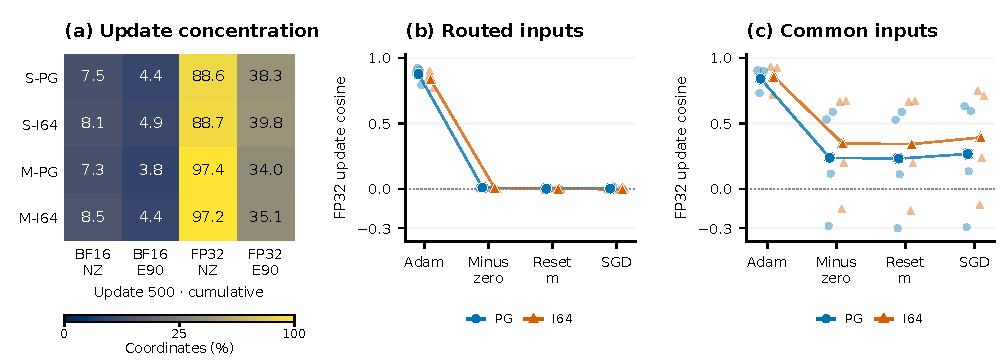
\includegraphics[width=\linewidth]{figures/nine_panel_20260914/section4_sparsity_overlap.pdf}
\caption{Parameter concentration and teacher-conditioned updates.
(a) Cumulative changes at update 500 for single-teacher (S) and joint (M) PG/I64 training, using DR. NZ is the nonzero coordinate fraction; E90 is the coordinate fraction carrying 90\% of squared change. Cells give percentages; color uses a square-root scale. S receives four times as many mathematics responses per update as M.
(b) At the common M-PG/500 student and optimizer state, FP32 top-1\% Jaccard versus signed update cosine. Small points average six teacher pairs within each bank; large points average four banks. Lines connect common-input (open) and routed-input (filled) conditions. SGD and reset-$m$ are individually norm-matched to saved-state Adam; circles denote PG and triangles I64.
(c) Teacher JS and $1-J$ on common inputs, with all six teacher pairs in all four banks. Colors and loss markers match (b); points share teachers and banks and are dependent. Updates use non-fused PyTorch steps on saved-state copies, rather than bitwise replay of the online optimizer.}
\label{fig:subnetwork_overview}
\end{figure}


\subsection{Shared Adam moments align teacher-specific updates}

Teacher-specific steps are strongly aligned at the update-500 sampled-token student with saved Adam state. We compare all six teacher pairs within each of four response batches, averaging pairs within a batch before averaging batches. Shared inputs hold prefixes fixed across teachers; domain-specific inputs use each teacher's own domain. On responses from each teacher's own domain, mean update cosines exceed 0.83 under both sampled-token and top-64 supervision. Resetting the first moment while retaining the second, or replacing Adam with norm-matched SGD, reduces the mean cosine to near zero (Figure~\ref{fig:subnetwork_overview}b). The accumulated first moment accounts for much of the alignment.

Adam's first moment can move parameters even with zero current gradient. To measure the change in a step induced by the current teacher gradient, we subtract this baseline. For update function $U(g;H)$ and saved state $H$,
\begin{equation}
\delta U_d=U(g_d;H)-U(0;H).
\label{eq:history_subtracted}
\end{equation}
Both steps start from identical parameters and optimizer state.

After this subtraction, the mean cosine between teacher-specific step differences falls below 0.01 on domain-specific inputs. When all teachers score the same prefixes, the residual cosine is larger, about 0.24--0.35 (Figure~\ref{fig:subnetwork_overview}c). Teacher-specific alignment therefore depends on both shared optimizer history and shared inputs: removing the zero-gradient component reveals much greater directional separation across domains.
